\documentclass{beamer}
\usepackage{listings}
\lstset{
%language=C,
frame=single, 
breaklines=true,
columns=fullflexible
}
\usepackage{subcaption}
\usepackage{url}

\usepackage{tikz}
\usepackage{pgfplots}
\pgfplotsset{compat=1.17}
\usepackage{tkz-fct}
\usepackage{mathrsfs}
\usepackage{txfonts}
\usepackage{tkz-euclide} 
\usetikzlibrary{calc,math}
\usepackage{float}
\newcommand\norm[1]{\left\lVert#1\right\rVert}
\renewcommand{\vec}[1]{\mathbf{#1}}
\providecommand{\pr}[1]{\ensuremath{\Pr\left(#1\right)}}
\usepackage[export]{adjustbox}
\usepackage[utf8]{inputenc}
\usepackage{amsmath}
\usetheme{Boadilla}
\titlegraphic{\includegraphics[scale=0.25]{IITHLogo.png}}
\title{Research Paper Presentation}
\author{Ramanathan Annamalai}
\institute{IIT Hyderabad}
\date{July 4, 2021}

\begin{document}
\begin{frame}
\titlepage
\end{frame}
\section{}
\begin{frame}{A Novel Model for Injecting Error in Probabilistic Gates}
\begin{block}{Abstract}
\begin{enumerate}
    \item Using inaccurate models to produce accurate results
    \item We will talk about developing an algorithm to a probabilistic gate model.
    \item Developing and calculating a metric for analysing accuracy - OPE.
    \item Simulating and Comparing simple and complex gates set-up used for the probabilistic model.
\end{enumerate}
\end{block}
\end{frame}

\section{Basics}
\begin{frame}{Few Terms}
\begin{enumerate}
    \item Electronic Design Automation (EDA) - Used for designing, simulating and verification of electronic systems such as integrated circuits and printed circuit boards.
    \item Stochastic Computational Models (SCM) - Stochastic computing is a collection of techniques that represent continuous values by streams of random bits.
   \item PCMOS - Probabilistic complimentary Metal Oxide Semiconductor.
\end{enumerate}
\end{frame}

\section{Logic Gates}
\begin{frame}{Logic Gates}
\begin{figure}
    \centering
    \includegraphics[width=\columnwidth]{LogicGates1.png}
    \caption{Basic Logic Gates and their Truth Tables}
    \label{fig:my_label}
\end{figure}
\end{frame}

\section{Introduction}
\begin{frame}{Efficiency}
\begin{block}{Understanding the output requirements}
\begin{enumerate}
    \item Many features need to be granted in the next computing system according to the target application.
    \item To get the better usage of the system, it is important to understand the application’s requirements as some applications can tolerate some error in their arithmetic blocks to get low-power consumption
\end{enumerate}
\end{block}
\begin{block}{Example}
Allowing about 5\% loss in classification accuracy for k-means clustering algorithm can lead to 50X improvement in energy saving compared to the fully accurate classification.
\end{block}
\end{frame}

\begin{frame}{EDA}
\begin{block}{}
\begin{enumerate}
    \item The conventional EDA tools employ deterministic methods to simulate the circuits by controlling the inputs and observing the outputs.
    \item The evolution in the integrated circuit (IC) industry and computing systems adds more complexity and challenges for EDA as there are many sources of error in the input values in real time.This has to be accomodated in simulations too.
\end{enumerate}
\end{block}

\end{frame}

\begin{frame}{Using Probability in EDA Simulations}
\begin{block}{}
\begin{enumerate}

    \item Using probability and allowing some error in the final result of the simulation will reduce the time taken for each simulation significantly.
    \item There are many probabilistic methods used in different areas of EDA tools to measure the circuit reliability, and the process variation on ICs manufacturing.
    \item Some computational methods like SCM and PCMOS use probability to arrive at their results.
    \item We will mainly be looking at comparing the probabilistic models with the accurate models and analyse the differences and feasibility of usage of such probabilistic methods.
    
\end{enumerate}
\end{block}

\end{frame}

\section{OPE}
\begin{frame}{Inaccurate Model}
\begin{enumerate}
    \item The accurate and inaccurate model accepts the inputs $in_1 (i) , in_2 (i)$ from the database. 
    \item An additional data set pertaining to the error $\epsilon$ is taken by the the inaccurate model.
    \item This $\epsilon$ may or may not be related to the data set or the gates which operate on them. For Probabilistic gates, the $\epsilon$ is an independent known probability distribution like uniform, exponential, normal, etc.
    \end{enumerate}
\end{frame}

\begin{frame}{Effect of $\epsilon$ on Logic Gates}
Based on the value of $\epsilon$, each logic gate changes it's behavior as shown in the below truth table.
\begin{figure}
    \centering
    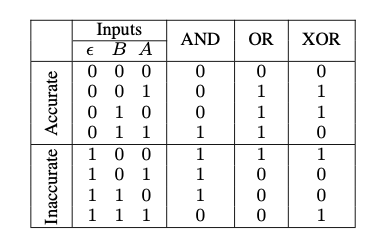
\includegraphics[scale=0.5]{TruthTable.png}
    \caption{Truth Table for AND, OR, XOR gates with $\epsilon$}
    \label{fig:my_label}
\end{figure}
\end{frame}

\begin{frame}{OPE Model}
\begin{figure}
    \centering
    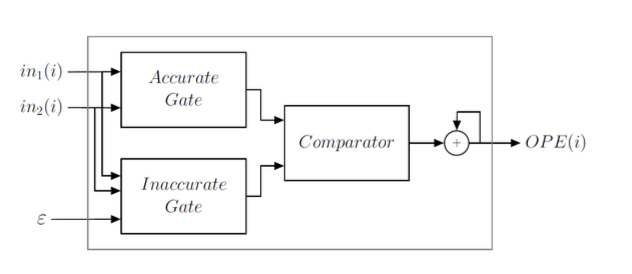
\includegraphics[scale=0.5]{OPE Model.png}
    \caption{OPE Calculation Model}
    \label{fig:my_label}
\end{figure}
\end{frame}

\begin{frame}{OPE Model}
\begin{block}{OPE}
\begin{enumerate}
    \item OPE is the Output Percentage Error. It is the average error produced in the inaccurate gate.
    \item To calculate OPE, we have a comparator device which compares the outputs of the accurate and inaccurate gates and takes the average error over the total inputs of the data set, say $N$, by using the below formula\\
    \begin{center} OPE = $\bigg( \frac{\sum_{i=0}^{N} {|{out(i)_{acc} - out(i)_{inacc}|}}}{N}\bigg) * 100\%$
    \end{center}
    \item $\epsilon$ can be considered as a PDF and OPE can be considered as it's equivalent CDF.
\end{enumerate}
\end{block}
\end{frame}

\section{Probabilistic Model}
\begin{frame}{Probabilistic Gate Model}
    \begin{block}{Components}
    \begin{enumerate}
        \item Accurate Gate - Defines the main required functionality of the model based on its inputs.
        \item Comparator - outputs $\epsilon$ by comparing the desired probability of error in our model and the estimated physical noise.\\The result of comparator depends on the probability distribution function of the noise.
        \item Multiplexer - Outputs either the result of the accurate gate or it's inversion based on the output of the comparator.
    \end{enumerate}
    \end{block}
\end{frame}

\begin{frame}{Probabilistic Model}
\begin{figure}
    \centering
    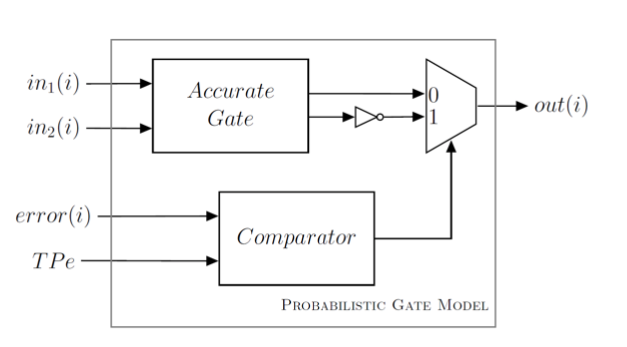
\includegraphics[scale=0.5]{ProbabilisticGateMode.png}
    \caption{Probabilistic Gate Model}
    \label{fig:my_label}
\end{figure}
\end{frame}

\begin{frame}{Probabilistic Gate Model}
    \begin{block}{Error Terms}
    \begin{enumerate}
        \item Physical error in the device (error) - Probability distribution function of the physical error.
        \item Target Probability Error (TPE) - related to the target number of outputs forced to be incorrect for a set of inputs. 
        \item Error in Probabilistic Model ($\epsilon$) - Function of physical error and TPE.
    \end{enumerate}
    \end{block}
\end{frame}

\begin{frame}{Probabilistic Gate Model}
    \begin{block}{Working}
    \begin{enumerate}
        \item Within a specific time t, the logic gate has a finite number of inputs and outputs n. 
        \item According to the error distribution and the probability of error, our model forces the output to be correct or incorrect.
        \item The exact series of steps involved is clearly explained in the Algorithm in the following page.
    \end{enumerate}
    \end{block}
\end{frame}

\begin{frame}{Probabilistic Gate Model}
    \begin{block}{Algorithm}
    $n$ \leftarrow \text{Number of Samples within Time t}\\
    \textbf{Inputs:}\\
        $\: in_1 (i) , in_2 (i) \in [0,1] $ \leftarrow \text{Time Space Inputs}\\
        $\:error(i)\in [0,1]$ \leftarrow \text{Time Space Physical Error}\\
        $\:Pe \in \{0,1\}$ \leftarrow \text{Probability of Error}\\
        $\:in_{th} \in [0,1]$ \leftarrow \text{Input Threshold}\\ \\
    \textbf{for}$(i \leq n)$ \textbf{do}
        \textbf{    if} $(in_1 (i) \leq in_{th})$ \textbf{then}\\
        $\quad crispin_1 (i) \leftarrow 0$\\
        \textbf{    else}\\
        $\quad crispin_1 (i) \leftarrow 1$\\
        \textbf{    end if}\\
    \end{block}
\end{frame}

\begin{frame}{Probabilistic Gate Model}
    \begin{block}{Algorithm Contd.}
 \textbf{    if} $(in_2 (i) \leq in_{th})$ \textbf{then}\\
        $\quad crispin_2 (i) \leftarrow 0$\\
        \textbf{    else}\\
        $\quad crispin_2 (i) \leftarrow 1$\\
        \textbf{    end if}\\
        $correct(i) \leftarrow crispin_1 (i) \textbf{logic operator} crispin_2 (i)$\\
        $incorrect(i) \leftarrow \textbf{NOT} (correct(i))$\\
        \textbf{    if} $(error (i) \leq Pe)$ \textbf{then}\\
        $\quad out(i) \leftarrow incorrect(i)$\\
        \textbf{    else}\\
        $\quad out(i) \leftarrow correct(i)$\\
        \textbf{    end if}\\
        \textbf{end for}\\
    \end{block}
\end{frame}

\section{Simple and Complex Gates}
\begin{frame}{Simple and Complex Gates}
    \begin{block}{Simple Gates}
    These are single gates producing outputs based on the inputs and errors as mentioned in the probabilistic gate models.
    \end{block}
    \begin{block}{Complex Gates}
    \begin{enumerate}
        \item These are combination of many simple gates, each of which behave in a probabilistic manner.
        \item The output of the complex gates is the result of inaccuracies in each simple gate.
        \item In this presentation we will mainly be focusing on the XOR topology, i.e. the arrangement of gates which produce an identical truth table to that of the XOR truth table.
    \end{enumerate}
    \end{block}
\end{frame}

\begin{frame}{Complex Gates}
    \begin{block}{Terminologies}
    \begin{enumerate}
        \item Topology - A particular arrangement of simple gates.
        \item Gate Count - Total number of gates in the set-up.
        \item Level - set of all gates which receive a common input.
        \item Structure - Either symmetric or non-symmetric based on the inputs of each gate in the same level. 
    \end{enumerate}
    \end{block}
\end{frame}

\begin{frame}{XOR Topologies}
\begin{figure}
    \centering
    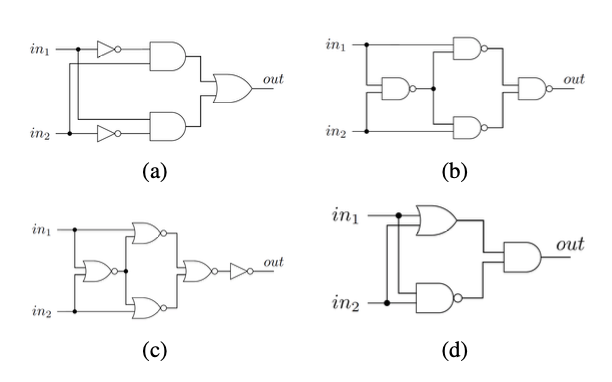
\includegraphics[scale=0.5]{XOR.png}
    \caption{Few XOR Topologies}
    \label{fig:my_label}
\end{figure}
\end{frame}

\begin{frame}{Complex Gates}
    \begin{block}{Characteristics of XOR Topologies}
    \begin{table}[]
        \centering
\renewcommand{\arraystretch}{1.4}
        \begin{tabular}{|c|c|c|c|}
        \hline
             Topology& Gate Count& Structure& Levels \\ \hline
             a& 5& Symmetric& 3\\ \hline
             b& 4& Symmetric& 3\\ \hline
             c& 5& Symmetric& 4\\ \hline
             d& 3& Non-Symmetric& 2\\\hline
        \end{tabular}
        \caption{Characteristics of XOR Topologies}
        \label{tab:my_label}
    \end{table}
    \end{block}
\end{frame}

\section{Simulations}
\begin{frame}{Simulations}
    \begin{enumerate}
        \item Now, we asses the probabilistic gates.
        \item We apply uniform and normal distributions by generating sufficient number of random data and fit the probability distribution function to these data.
        \item For the normal distribution, the applied data has $\mu = 0.5$ and $\sigma = 0.125$.
        \item As there is no control on the physical error in the real device, we sweep $Pe \in [0,1]$ to get the result of OPE.
        \item OPE is calculated over $Pe$ range to check the effect of the added noise on simple and complex gates.
    \end{enumerate}
\end{frame}

\begin{frame}{Simulations}
    \begin{block}{Simple Gates}
    \begin{enumerate}
        \item $P(0)$ is the probability of correct '0' output, and $P(1)$ is the probability of correct ’1’ output.
        \item These probabilities are proved to be exact to the accurate gate in case of $Pe = 0$, and inverted for $Pe = 1$.
        \item The results of OPE are found to be identical with CDFs of fitted PDFs for the injected noise either as uniform or normal distribution.
        \item OPE for simple gates is independent of the functionality of these gates, as it is only effected by the noise distribution in the gate. 
        \item OPE equation can be re- written as:\\
        \begin{center}
            OPE = $\bigg(\displaystyle \sum_{i\leq Pe}^{} \frac{|error_i|}{N}\bigg) * 100\%$
        \end{center}
    \end{enumerate}
    \end{block}
\end{frame}

\begin{frame}{Simulations}
\begin{block}{Simple Gates Graph}
\begin{figure}
    \centering
    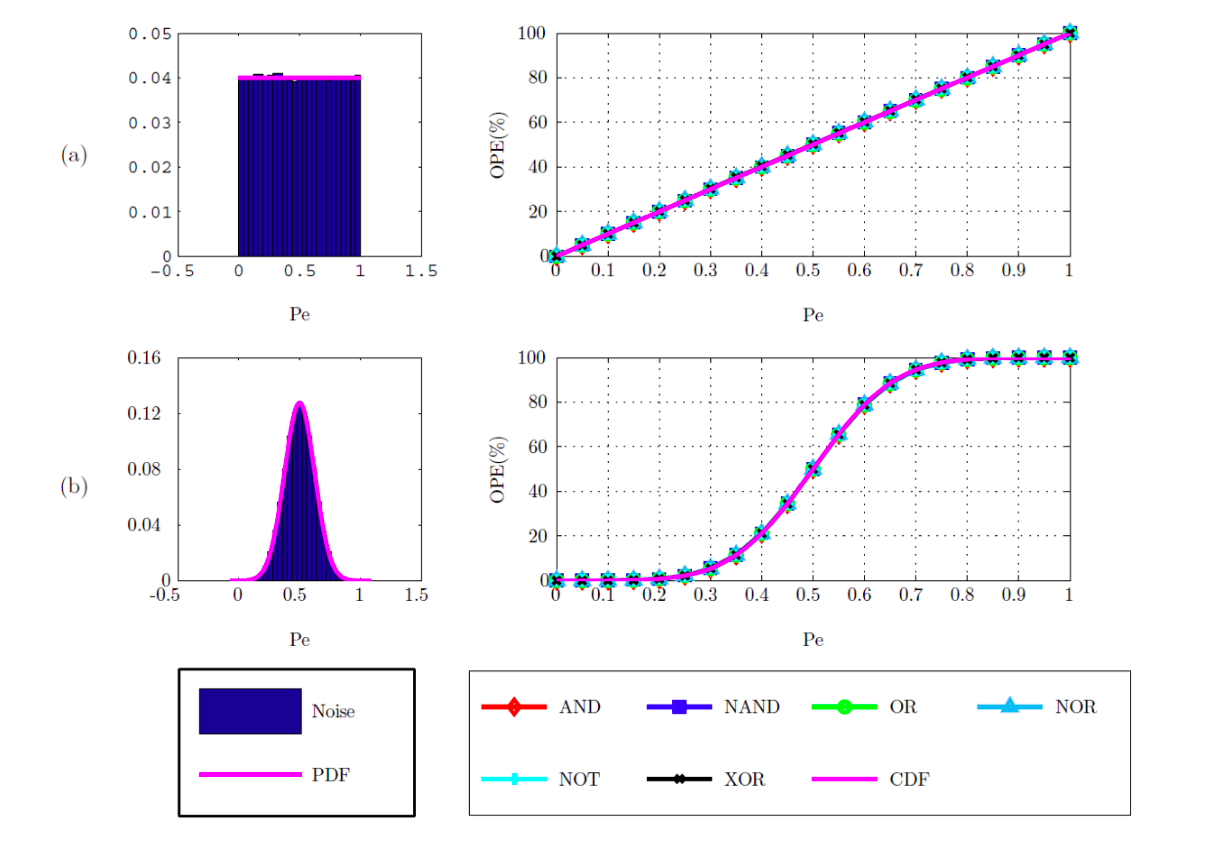
\includegraphics[scale=0.2]{SimpleGateSimulations.png}
    \caption{OPE for simple gates, and CDF of the injected noise (on the right) and Histogram of the injected noise with the fitted PDF of it (on the left) are plotted for, (a) Uniform Distribution, and (b) Normal Distribution}
    \label{fig:my_label}
\end{figure}
\end{block}
\end{frame}

\begin{frame}{Simulations}
    \begin{block}{Complex Gates}
    \begin{enumerate}
        \item The results for complex probabilistic XOR gates show great improvement in OPE for $Pe \geq 0.5$ and little degradation in the performance for $Pe \leq 0.5$.
        \item First and second topologies have the same OPE despite the difference constellation cause of OPE is identical between each level in first topology with its analogous level in second topology as shown in both distributions.
        \item Third topology which has the largest level of gates and the highest count has the best OPE among other topologies because of the last NOT gate in the constellation which has the great impact on OPE improvement.
    \end{enumerate}
    \end{block}
\end{frame}

\begin{frame}{Simulations}
    \begin{block}{Observations in Complex Gates}
    \begin{enumerate}
        \item Topologies with even levels as topology c,d show better OPE rather than that with odd levels as topology a,b.
        \item All levels of gates in the XOR topologies have the same OPE.
    \end{enumerate}
    \end{block}
\end{frame}

\begin{frame}{Simulations}
\begin{block}{Complex Gates (XOR) Graph}
\begin{figure}
    \centering
    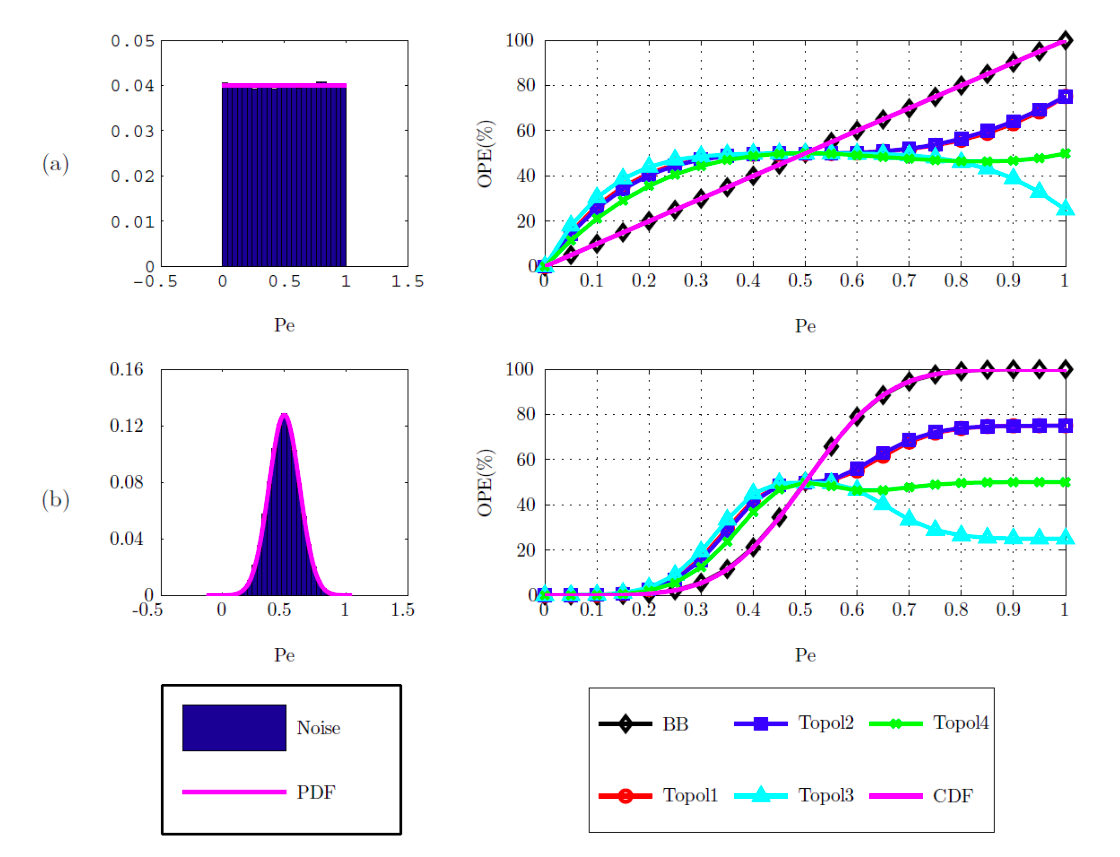
\includegraphics[scale=0.2]{ComplexGateSimulations.png}
    \caption{OPE for different XOR topologies, and CDF of the injected noise (on the right) and Histogram of the injected noise with the fitted PDF of it (on the left) are plotted for, (a) Uniform Distribution, and (b) Normal Distribution}
    \label{fig:my_label}
\end{figure}
\end{block}
\end{frame}

\section{Summary}
\begin{frame}{Summary}
    \begin{enumerate}
        \item The primary purpose of this paper is developing an algorithm to model probabilistic gates which is implemented by a device with an error that can be extracted as a probability distribution function.\\\\
        \item This can be useful in modeling probabilistic gates in EDA tools.\\\\
        \item This model is investigated for simple and complex gates by applying uniform and normal random distribution as error for these gates.\\\\
    \end{enumerate}
\end{frame}

\begin{frame}{Summary}
    \begin{enumerate}
        \item Using the OPE for numbers of inaccurate samples as a metric to measure our model’s efficiency proves validation of the model, as OPE for simple probabilistic gates matches CDF of injected noise for uniform and normal distributions.\\\\
        \item Integrating these simple gates to implement four different complex topologies of XOR gate, and study the effect of simple probabilistic gates on XOR functionality shows OPE improvement in topologies with even levels.\\\\
    \end{enumerate}
\end{frame}

\end{document}
